\documentclass{article}%
\usepackage[T1]{fontenc}%
\usepackage[utf8]{inputenc}%
\usepackage{lmodern}%
\usepackage{textcomp}%
\usepackage{lastpage}%
\usepackage{authblk}%
\usepackage{graphicx}%
%
\title{Differential Effects of Collagen Prolyl 3{-}Hydroxylation on Skeletal Tissues}%
\author{Jack Oliver}%
\affil{Laboratory of Tumor Biology, Angiogenesis and Nanomedicine Research, National Center for Cell Science, Pune, India}%
\date{01{-}01{-}2013}%
%
\begin{document}%
\normalsize%
\maketitle%
\section{Abstract}%
\label{sec:Abstract}%
Researchers at Southern California Institute of Technology have developed a biomimetic peptide modeled after crustaceans and pigs to remedy some of the ills of the world's oceans. The peptide is an enzyme that, when multiplied, forms tiny calcium carbonate caps that promote a normal immune response to invading organisms.\newline%
The researchers describe their research in this week's edition of Proceedings of the National Academy of Sciences (PNAS).\newline%
"As plastic materials expand, they create lesions in the sea floor and climate change will make these lesions more prominent and cause more severe ills than we had thought possible," said Christopher Meijer, an assistant professor of molecular biosciences at USC and an investigator in Southern California Institute of Technology's developmental biology laboratory. "This work could solve some of the most severe conditions that we suffer from as a result of our ubiquitous plasticity."\newline%
Meijer and colleagues think that the oligopigestin receptor 4{-}dependent peptide is a good candidate for new organisms that might tolerate the added ecological hazards of plasticity. This compounds could prompt the creation of more ecologically appropriate organisms, including "crops" with room for runoff into the sea. Meijer said that the resultant ocean organisms could protect other organisms from damage.\newline%
Meijer collaborated with Charles Cheng, Associate Professor of Biomimetics at USC, and senior investigator Daren van der Hub of the Naval Research Laboratory (NRL) in Pasadena. The research was funded by the National Science Foundation.

%
\subsection{Image Analysis}%
\label{subsec:ImageAnalysis}%


\begin{figure}[h!]%
\centering%
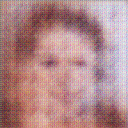
\includegraphics[width=150px]{500_fake_images/samples_5_166.png}%
\caption{A Man In A Suit And Tie Holding A Toothbrush}%
\end{figure}

%
\end{document}